\section{N2Sky Architecture}\label{TheN2SkyArchitecture}

\subsection{Current Architecture Analysis}\label{CurrentArchitectureAnalysis}

The current N2Sky architecture is a monolithic standalone application, heavily maintainable and not scalable. Before proposing the new architecture design, it is important to find the weak parts of the current application and define which functionalities are still reusable. By doing that, new functionalities in a reasonable time will be gained.

\subsubsection{Architecture Design}\label{Architecturedesign}

The current N2Sky design is based on RAVO architecture \cite{ravo}, which extends default SPI stack. SPI stack contains Infrastructure as a Service (IaaS), Platform as a Service (PaaS) and Software as a Service (SaaS). The architecture had two phases of integration. In the first phase, the SPI was extended and applied to the N2Sky application. On the last phase, all mandatory components were implemented and integrated as presented in figure \ref{fig:current_arch}.

\begin{figure}[htbp]
\begin{center}
  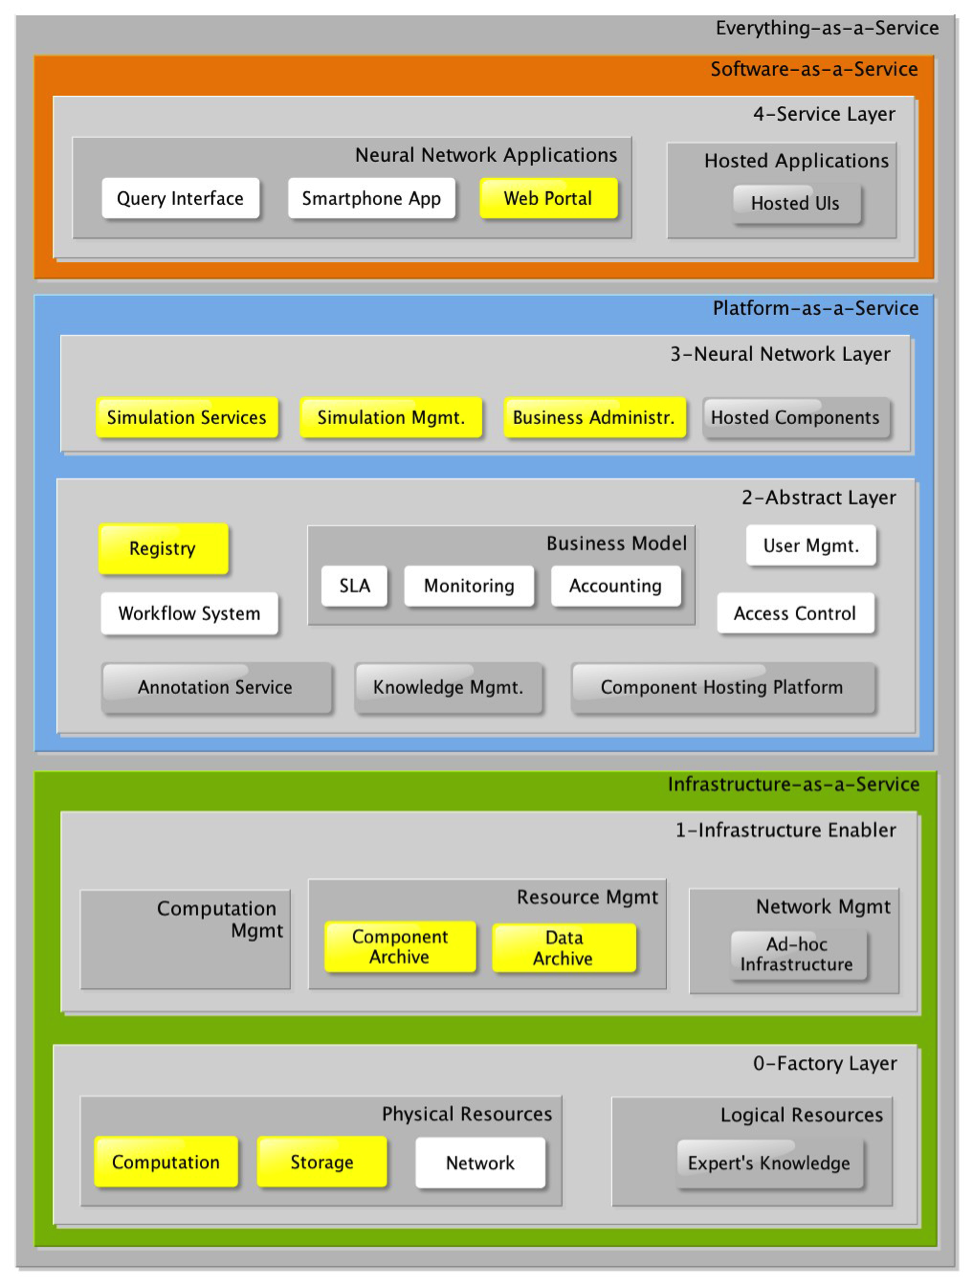
\includegraphics[width=\linewidth]{components/2/current_arch.png}
  \caption{Current N2Sky architecure}
  \label{fig:current_arch}
\end{center}
\end{figure}

Every service represents a particular layer:
\begin{itemize}
\item \emph{IaaS layer}  responsible for managing the resources. It contains the logical and physical resources of N2Sky components as well as infrastructure enabler like protocols, procures etc. 
\item \emph{PaaS layer}, which provides an access to resources via API. In the previous N2Sky system, it served as a domain-independent tool. It also contains the neural network layer.
\item \emph{SaaS} is a service, which contains the User interfaces (UIs).
\end{itemize}

Everything as a service is considered to be a good idea but build upon it, the layered architecture could cause various issues. Since every layer is depending on the above one, there exists a possibility that if the services from the bottom layer are unreachable, then the application is not usable at all. 

Besides the stand-alone-application design, which was implemented, another issue is encapsulation. Since every service needs to communicate with other services via API, the order of layers could be violated. This problem can cause not only security issues, bus also consistency, namely it can break the desired workflow process.

Unfortunately, it is impossible to distribute the services, since they are all coupled together into a collection of layers.  

\subsubsection{Components}\label{Components}

N2Sky was an imposing application, working as a whole which contained multiple services. These main components were listed in N2Sky:

\begin{itemize}
\item \emph{The component archive} was responsible for storage and file management.
\item \emph{The data archive} is the component, which managed the neural network specific resources in XML and JSON formats. 
\item \emph{The registry}, which was a base component of the N2Sky architecture. This component was responsible for searching for services within the cloud.  It also contained instructions and rules, used by users. 
\item \emph{Monitoring} was divided into two subcategories: business activity monitoring (BAM), which gathered the business data and technical monitoring, which was responsible for environmental monitoring and performance statistics. 
\end{itemize}

Considering that the registry is a central component, responsible for services management, it can slow down the whole process. All requests go throw this service. If the services are not accessible and high latency or waiting time occur, the UI as well as the API services would be unavailable.

Having the same services distributed on multiple servers would be great. Every service in the previous version of N2Sky is gigantic, that is why it is possible to divide services into microservices and incapsulate sensible components from public access.


\subsubsection{Implementation}\label{Implementation}

The previous version of N2Sky is fully written in Java using Spring framework, Java servlets and Tomcat server. The Java Spring framework is best used for enterprise applications, but N2Sky needs lots of computations so the high-end supercomputers are a necessary pre-requirement in this case. 

Unfortunately, it is impossible to map the current architecture into the microservices approach. The only solution is making replicas of the application, but then the sessions and data consistency have to be tracked in each one of them.  

The mobile application of N2Sky is built in raw HTML5 and JavaScript. Today, looking on this mobile application, is almost impossible to maintain it. Nevertheless, the mobile version is also wrapped into a layered architecture, while the implementation part is still one project. The solution to this problem is the responsive design. The responsive design could be fully adaptive to multiple devices from desktop PCs to mobiles with a small screen resolution.

The whole system is deployed on Amazon Web Services (AWS), which is a good thing if the owner has enough resource to keep it working. The best solution would be to have a dedicated server with a real physical memory and computational abilities.  


\subsubsection{Usability and User Experience}\label{Usabilityanduserexperience}



\subsection{Redesign Motivation}\label{Redesignmotivation}

Application redesign is a project, which takes a lot of work and time. But at some point, every designer has faced a refactoring project. It is strongly connected to the user experience. Bad user experience will make users stop using an application and leave negative feedback for the application. 

\subsubsection{Redesign Process }\label{Redesign Process}

There is available data, information and user experience of the previous version of N2Sky to work with. During the redesign, it was already known who the users are and what they are trying to achieve. Using such information, the possibility to create future goals for user interface and user experience is high.


\begin{description}

\item[Finding problems.]  There are multiple problems with the application. One of the most crucial is that the user interface is not intuitively understandable as it shown in figure \ref{fig:old_arch}. 
\begin{figure}[htbp]
\begin{center}
  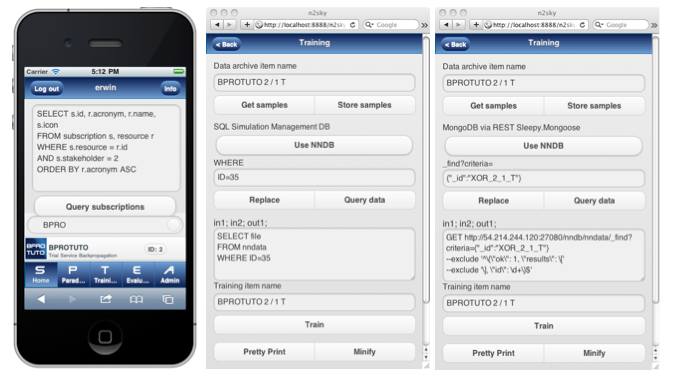
\includegraphics[width=\linewidth]{components/2/old_arch.png}
  \caption{Current N2Sky User Interface}
  \label{fig:old_arch}
\end{center}
\end{figure}


After signing in, to the user is shown a subscription form, paradigm services and paradigm metadata views without any description field. Small titles are unfortunately not always self-describing. The application is in general oriented on that group of users, who comes from the IT area. In some forms, queries can be typed, but the type-safe fields and no autocomplete are missing.
The representation of a neural networks trained model is not readable. The model is represented as a raw JSON or XML file and the user cannot download it. The last point is the general design, which does not look up-to-date and user attractive. 


\item[User interviews and Questionnaire.]
User insights are very important. They help with the understanding of problems nature. In the case that a user finds something confusing, the interviewer needs to dig deeper to stress the importance of particular insights. Unfortunately, there were no analytic data or any reviews regarding UI and UX. With a small group of colleges, the current UI of N2Sky was reviewed. 
The following questions were derived (Q1-Q5): 


\begin{itemize}
\item Q1: "How can N2Sky help you with the developing of your neural network?"
\item Q2: "What was the most difficult part of creating a new model?"
\item Q3: "Did you face any problems during spawning of your neural network? If yes, what kind?"
\item Q4: "Did you find out something new, when other users were performing testing against your neural network?"
\item Q5: "What did you miss during the using of N2Sky?"
\end{itemize}    

There were five students interviewed which were grouped together. The summarised answers (A1-A5) according to questions (Q1-Q5) are shown below: 

\begin{itemize}
\item A1: N2Sky gives the possibility to test the own neural network. Unfortunately, if the user does not have a neural network it is impossible to test the application.   
\item A2:  A user faces difficulties during the creation of a new neural network model. The user interfaces contains technical jargon and it is not intuitively understandable.  
\item A3:  Spawning a neural network was a pretty clear process, but it was unclear if the neural network was ready to be used or not.
\item A4:  Logging of the training data is very useful. The neural network owner can see how his network behaves with different training and testing data.
\item A5:  A user would want to perform testing and training on already existing neural networks. 
\end{itemize}    


\item[Current application design mapping.]

After studying the answers, highlighting weak parts of the application was easier. This approach will show a big picture of the current application design:

\begin{itemize}
\item An arbitrary user needs to know multiple technologies and programming languages just to simply reuse existing neural networks. 
\item Too much information on every view. The purpose of the view is overloaded. Each view has too much functionality, which makes the user loose focus.
\item The application works relatively slow. Even if processes behind might be happening, the user does not know it.
\end{itemize}

Important is to face the problems, but that does not "reinvent the wheel".  As Joel Spolsky the founder of Netscape and CEO of Stack Overflow said: "throwing away the whole program is a dangerous folly" \cite{joel}. That is why it was decided to consider the problems of current N2Sky design and reuse working ideas in a refactored system

\item[Application Maintenance.]
N2Sky was the monolithic standalone application, which included all services in one and was deployed as a whole. The application was not distributed. In case one of the services did not work correctly, the whole application was unusable. 
Originally the previous version of N2Sky was fully written in Java. There were hundreds of classes, providers, and services in one project. The developer would spend hours to maintain this kind of project. Finding an issue in a big application is always a challenge. Small changes are causes for subsequence changes. If the software breaks after such a change, then it will add high effort for fixing it. As Robert Cecil Martin wrote in his book "Clean Code": "The code is hard to understand. Therefore, any change takes additional time to first re-engineer the code and is more likely to result in defects due to not understanding the side effects" \cite{cleancode}.  He categorizes this kind of code as "Smell" code. Unfortunately, seen from the maintaining perspective, N2Sky had all the above mentioned problems.

That is why N2Sky has shifted from a monolithic system to a container based system with an independent micro service which located in the cloud environment. 
The frontend and its services are lightweight and easy maintainable. If something happens to go wrong, the developer will know exactly where the problem is. The independence of services makes it almost impossible to break something during fixing it. 
Additionally, there are monitoring and alerting systems which support developers during maintenance. Before, a user could not tell it the application was working correctly or was it even running. Users could get a bad experience while using an application in case of an improperly working environment. Now, it is possible not only to notify an application administrator about problems but also to predict potential threads. 
\end{description}


\subsubsection{Refactoring the User Interface}\label{Refactoring the User Interface}

User Interface (UI), an abbreviation of the user interface, allows the interaction of a user with a program through graphical visualization made by text, icons, buttons, and pictures. While deciding the design of a user interface there are some highly recommended features also known as heuristics, which were invented by hl{Jakob Nielsen}. It was decided to apply the following ten general principals of interaction design to N2Sky:

\begin{itemize}
\item \emph{Simple and natural dialogue.} N2Sky will have a simple UI which is understandable for any user, even if the user is not an expert. Every icon, navigation or action button will be self-describing. The application will follow the slogan "less is more". No more overloaded views. The idea of the N2Sky UI design is that one particular view is responsible for one particular function or group of functions which are coupled tight together.
\item \emph{Speak the user's language.} Developing N2Sky was concentrated on user perspective. There is no technical jargon for the arbitrary user.
\item \emph{Minimize user memory load.} There is no multiple options, functions or menus in one view. There is also no multiple ways to do the same thing. N2Sky teaches the user how to make things done with one existing and convenient workflow. 
\item \emph{Consistency.} N2Sky has similar layouts, fonts, colors, icons types, structures and organization through the entire application. The user should get the same visual experience in every view.
\item \emph{Feedback.} Every action, process or even error will be notified. The user will know exactly what is happening with the system with clear and understandable messages.
\item \emph{Clearly marked exits.} Every push-to-action button has a short and clear caption.
\item \emph{Shortcuts.} N2Sky has multiple user types. One of the types is the expert user, which is the advanced user in neural network and artificial intelligence topics. For this kind of user is provided more technical jargon, but this UI is separated from arbitrary users UI.  
\item \emph{Good error messages.} Every notification is understandable and includes an error message if it happens to occur. Every message has a simple description.
\item \emph{Prevent errors.} In N2Sky is implemented the logical structure of UI components. There are constraints which help the user in the workflow. For example, the user will always get a default value of any input.
\item \emph{Help and documentation.} N2Sky will have tutorials that describe the user workflow. The expert users will also get an API documentation with a detailed description and sample requests. 

\end{itemize}

Each and every one of these heuristics is connected to a crucial idea that is usability. By mentioning this idea, a straightforward relationship with the UX follows since this is also one of the key concepts that grows along the rapid development of technology. UX is known as user experience and it describes the perspective and feelings a user gets when interacting with the product. It deepens into such aspects as the users inner circumstances and the nature of the created design. The goal is to achieve such a system that offers distinguished user experience and accomplishes the most of aspects \cite{uixagenda}.
Putting both of UI and UX in comparison, to all appearances the user interface is the target of the appearance and functionality of the product and its tangible details.  Furthermore, the user experience is the general experience that the user manages throughout the whole use. 
UI will concentrate on the appearance and design of the product, rather than the functionality. The intent of it relies on the visual design and layout. UI covers issues such as how a button is supposed to look like, how the errors are going to appear or the visually comprehensibility meaning which colors or font type shall be used for a better perceptibility of the product \cite{humanpc}. 
UX points its focus on the involvement of the user while interacting. It is measured by a variety of tests and researches done to achieve a higher satisfaction on the users side.
Though their differences, the only matter which relates both UI and UX is their priority, in other words, the user. When expanding the concept of both these definitions it can be concluded that one co-exists with the other. There would not be user interface without user experience and vice versa. 

\subsubsection{Advanced Project Management}\label{Advanced project management}

In order to make N2Sky competitive on the market, a modern approach in the planning of the project has to be done. Today the most common and effective way in development and planning is well-constructed Functional Requirements Specification (FRS), which helps to estimate effort and advice in future planning. 

FRS is a document that defines functionality, which the application or some parts of it must perform \cite{wiki:frs}. N2Sky is a sociotechnical system, meaning that it strongly interacts with humans. 

FRS for N2Sky is described in the natural language with formal methods in order to establish specifications between development process and end-user consuming. Every N2Sky module has FRS, which is explicit and points on the systems functionality. A good FRS must be unambiguous, consistent and correct \cite{frs_1}.  
 
The formal or semi-formal methods serve for analyzing and validating FRS. The main purpose of that is to limit interpretation errors. The problem occurs when FRS is fully written in natural language when designers do not have required technical knowledge in order to use other languages. One of the typical solutions is that it defects detection techniques, which require effort from the designer \cite{frs_3}. 
 
In N2Sky, some methods and techniques were applied in order to make specification as clean and clear as possible. Despite that, in FRS will always be parts which are leading to misunderstanding \cite{frs_1}.
  
FRS is part of the engineering phase. Following qualities for N2Sky were defined and applied during this phase \cite{frs_4} as shown in figure \ref{fig:frs_req}:
\begin{itemize}
\item Correct
\item Unambiguous
\item Complete
\item Consistent
\item Ranked for importance and/or stability
\item Verifiable
\item Modifiable
\item Traceable 
\end{itemize}


\begin{figure}[htbp]
\begin{center}
  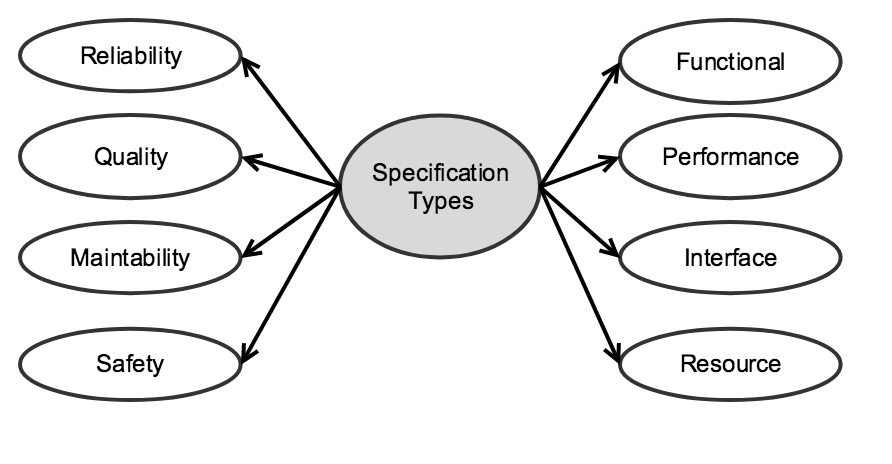
\includegraphics[width=\linewidth]{components/4/pics/frs_req.png}
  \caption{Requirement Specification Qualities}
  \label{fig:frs_req}
\end{center}
\end{figure}


\subsubsection{User Roles}\label{User Roles}

In order to make the N2Sky user interface understandable for arbitrary users as well as professional for advances users, it was decided to separate the user roles. Every user role has his own way of interaction with the application.

Every user has some specific area within the works. For example, authorised users do not need to know the current environmental monitoring information. These restrictions were the motivation to create some user roles in order to restrict or grand some functionality of N2Sky as shown in figure \ref{fig:userroles}.

\begin{figure}[htbp]
\begin{center}
  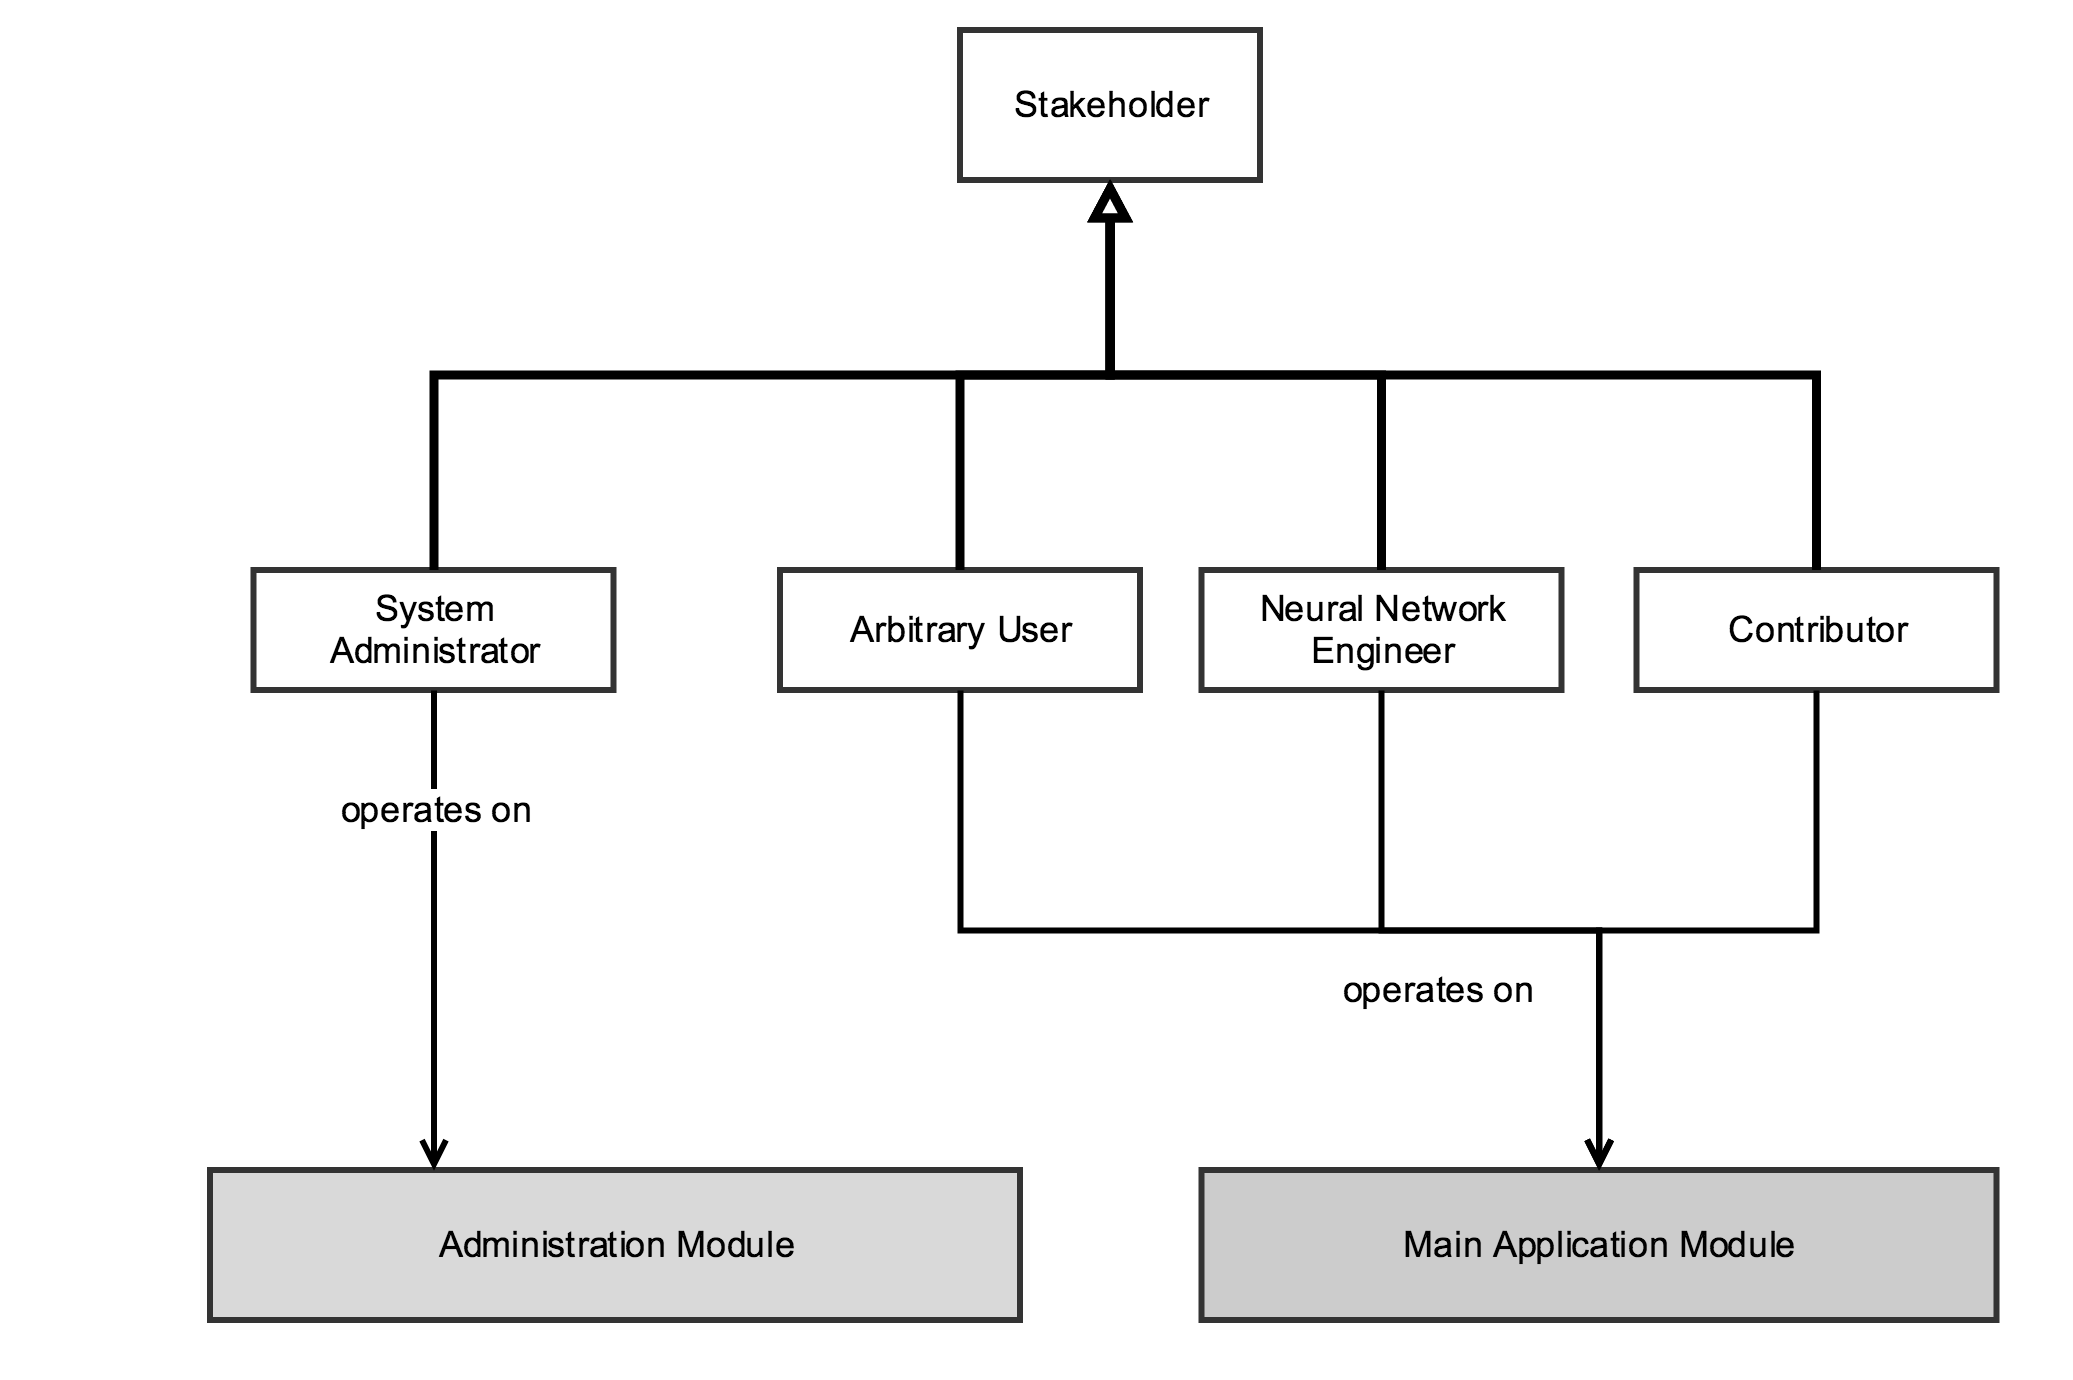
\includegraphics[width=\linewidth]{components/4/pics/users.png}
  \caption{User roles hierarchy and modules where they are operating on (marked grey)}
  \label{fig:userroles}
\end{center}
\end{figure}

\begin{itemize}
\item \emph{Arbitrary User.}  The Arbitrary User is a user, who does not have a deep knowledge of the neural network field or know any programming language. His main purpose is not a contribution, but the usage of already existing neural networks and trained models. The main goal of the arbitrary user is to study neural networks within N2Sky platform. The arbitrary user can also evaluate the trained models or execute training against existing neural networks. This kind of user does not have to use his own training data, he just wants to see the behavior of neural networks. The arbitrary user can be converted to a Neural Network Engineer user if he has enough knowledge for it. 
\item \emph{Neural Network Engineer.} The Neural Network Engineer is an arbitrary user. The Neural Network Engineer has access only to his own dashboard and publicly available resources on the main application module. He can perform the semantic search for available neural network paradigms and use them. This user can create his own neural network instances from existing neural network paradigms. He can also train the running neural network instances and evaluate their trained models. This user can share his trained neural network by making it public. 
\item \emph{Contributor.} The Contributor is an expert user, which has enough knowledge and experience to create his own neural network. This user can create neural network paradigms using the ViNNSL template schema and publish them on N2Sky. This user can deploy neural networks on the N2Sky environment as well as on his own environment by providing training and testing endpoints. The goal of the contributor is the study how his networks will behave with different network structures, input parameters and training data that is provided by other users.
\item \emph{System Administrator.} System Administrator is a user who has full access to the application including environmental management, monitoring and alerting features. The administrator can manage OpenStack and Cloudify instances. He also can shadow any N2Sky user to observe the application from other perspectives. The administrator has access to all dashboards in every module.
\end{itemize}


\subsubsection{User Main Functions}\label{User Permissions}

In the more detailed overview of user roles it is possible to define permission and main functions.
Permissions describe a users allowed page view. If the user has access to a particular page view, the main user function can be defined. 
The main user function characterizes allowed behavior on a particular page view. 

As it was mentioned in the previous chapter,  N2Sky is a modular application. Permissions and main functions of the Administration Module and N2Sky Main Application Controller, which is a part of Main Application Modules, are described in Table \ref{table:admin}.

\begin{table}[]
\resizebox{\textwidth}{!}{%
\begin{tabular}{|l|c|c|c|c|c|c|c|c|}
\hline
\multicolumn{1}{|c|}{User Role} & \multicolumn{2}{c|}{\textbf{Administration Module}}          & \multicolumn{2}{c|}{\textbf{N2Sky Main Application Controller}}      \\ \hline
\multicolumn{1}{|c|}{\textbf{}} & \textbf{OpenStack Management} & \textbf{Cloudify Management} & \textbf{Neural Networks Management} & \textbf{Trained Models Management} \\ \hline
System Administrator            & \textbf{+}                    & \textbf{+}                   & \textbf{+}                          & \textbf{+}                            \\ \hline
Moderator                       & \textbf{-}                    & \textbf{-}                   & \textbf{+}                          & \textbf{+}              \\ \hline
Consumer                        & \textbf{-}                    & \textbf{-}                   & \textbf{-}                          & \textbf{-}                            \\ \hline
Developer                       & \textbf{-}                    & \textbf{-}                   & \textbf{-}                          & \textbf{-}                               \\ \hline
Contributor                     & \textbf{-}                    & \textbf{-}                   & \textbf{-}                          & \textbf{-}                    \\ \hline
\end{tabular}%
}
\caption{User Roles main functions considering "Administration Module" and "N2Sky Main Application Controller". 
"+" for allowed, "-" for disallowed}
\label{table:admin}
\end{table}

System Administrator has permissions to all components. Moderator has access only to N2Sky Main Application Controller. Since both of this user role extending Contributor user role, the permissions for main application module are also granted.

Consumer, Developer, and Contributor user roles have no access to any administration parts of N2Sky. These users do not have any main function in this area, but they can operate N2Sky Main Application Module as it shown in Table \ref{table:main}.

\begin{table}[]
\resizebox{\textwidth}{!}{%
\begin{tabular}{|l|c|c|c|c|}
\hline
\multicolumn{1}{|c|}{User Role} & \multicolumn{4}{c|}{\textbf{N2Sky Main Application Module}}                                                                                    \\ \hline
\multicolumn{1}{|c|}{\textbf{}} & \textbf{Paradigm Creation} & \textbf{Neural Networks Creation} & \textbf{Neural Network Training} & \textbf{Training Models Evalutaion} \\ \hline
System Administrator            & \textbf{-}                 & \textbf{-}                        & \textbf{-}                       & \textbf{-}                          \\ \hline
Moderator                       & \textbf{-}                 & \textbf{-}                        & \textbf{-}                       & \textbf{-}                          \\ \hline
Consumer                        & \textbf{-}                 & \textbf{-}                        & \textbf{+}                       & \textbf{+}                          \\ \hline
Developer                       & \textbf{+}                 & \textbf{+}                        & \textbf{+}                       & \textbf{+}                          \\ \hline
Contributor                     & \textbf{-}                 & \textbf{+}                        & \textbf{+}                       & \textbf{+}                          \\ \hline
\end{tabular}%
}
\caption{User Roles main functions considering "N2Sky Main Application Module". 
"+" for allowed, "-" for disallowed}
\label{table:main}
\end{table}

As it was mentioned before, the System Administrator as well as Moderator has access to the N2Sky Main Application Module, but they do not have the main function over that. On the other hand, all user roles, which are extending consumers can contribute to the N2Sky Main Application Module, except Consumer itself. The consumer has access to all page views on this module, but he has another purpose. 



\subsection{Novel N2Sky Architecture}\label{Contemporary N2Sky Architecture}

N2Sky is a simulation platform, which allows all involved stakeholders to use it for computational purposes. In order to achieve high performance and scalability, it was decided to use the microservices architecture. This approach is used not only for backend services but also with frontend and its services.

The user-centered design is a fundamental requirement for N2Sky. Looking back on past experiences with the application, there were identified the real capabilities and needs of users. N2Sky was moved from a complex monolithic system to an easily understandable application. Every interested user without having deep knowledge in the neural network field can freely use N2Sky.  The goal was to save and gain the current functionality of the application and decrease the visual complexity of it. 

\subsubsection{Cloud Infrastructure}\label{Cloud infrastructure}


Upon the N2Sky microservices is located the load balancer, which includes shared cloud resources. Since the N2Sky environment needs to support thousands of Docker containers \cite{docker} simultaneously, only one container orchestration like Cloudify \cite{cloudify} with a microservices architecture could perform this.  Cloudify is a container orchestration tool, which provides communication between cloud platforms and manages container deployment and execution. Docker container is an operating-system-level virtualization. Containers technology is used across entire system from frontend and its services to monitoring and alert management system. 

The novel N2Sky architecture can be scaled horizontally as well as vertically on demand as presented in figure \ref{fig:newarch}.

\begin{figure}[H]
\begin{center}
  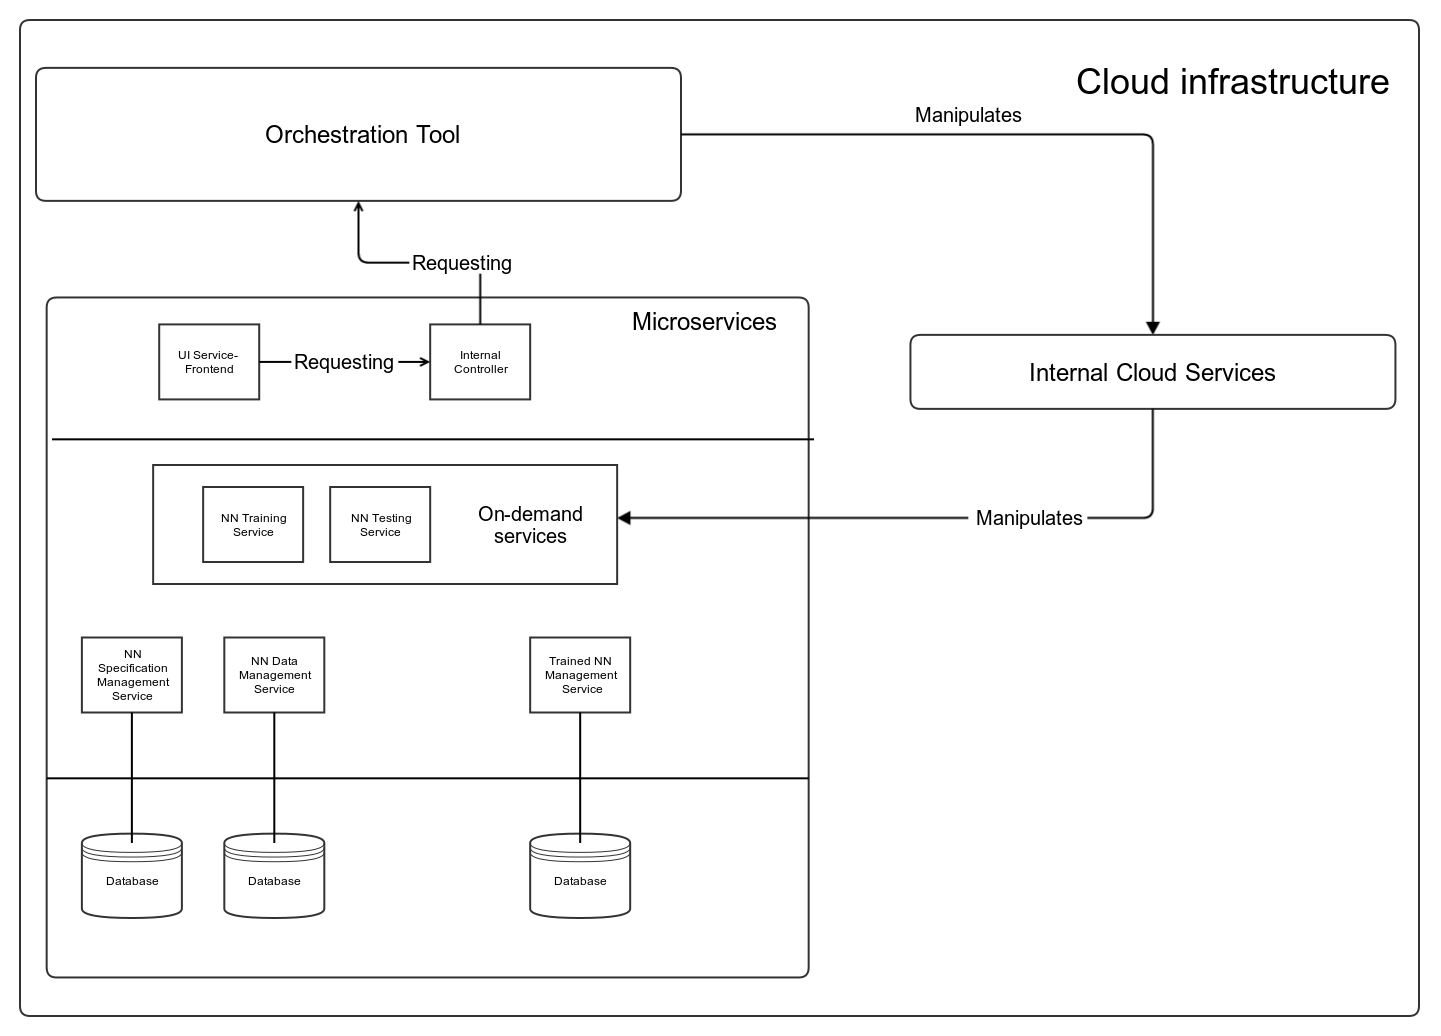
\includegraphics[width=\linewidth]{components/2/architecture.png}
  \caption{Novel N2Sky Architecture}
  \label{fig:newarch}
\end{center}
\end{figure}

\begin{itemize}
\item \emph{Orchestration Tool} is the Cloudify framework, which communicates with a cloud infrastructure, namely creates and manages new instances. Every instance is a Docker container.
\item \emph{Internal Controller} is a service, which works directly with the Cloudify tool. This service handles user request in order to create, delete or update Docker containers.
\item \emph{UI Service-Frontend} is a modular application. The user can request container management over the UI, which will be redirected to Internal Controller.
\item \emph{On-demand services} are not exposed publicly, which can be controlled only by internal web services.  This approach helps to encapsulate the services pool, which increases security in the entire application. 
\item \emph{Neural Network Specification Management Service}  is a service, which is responsible for controlling existing neural network paradigms, namely train, retrain and persist trained models.
\item \emph{Neural Network Data Management Service}, is located right on top of the database and provides the API for adding external data sources.
\item \emph{Trained Neural Network Management Service} is a service, which is responsible for evaluating trained models.
\end{itemize}


 
 
\subsubsection{Modular Frontend Application Design}\label{Modular frontend application design}

Maintaining such a large application like N2Sky with the monolithic approach is unwieldy. Since N2Sky supports the microservices approach in the backend, it was decided to apply the same solution on the frontend.  

Microservices in the frontend are small independent web applications, which are consolidated into one application. The main benefits of this approach are:

\begin{itemize}
\item \emph{Maintainability.} It is possible to divide application between different teams. Developers do not even need to have knowledge about other parts of the application. 
\item \emph{Diversity of technologies.} The monolithic approach makes the whole application stick to one framework. Microservices allow to use any technology without the need to rewrite the application.
\item \emph{Independent deployment.} Every application has release periods. Every release is accompanied with a redeployment procedure. There is no need to redeploy the whole application, but just only the required components.
\end{itemize}


\begin{figure}[H]
\begin{center}
  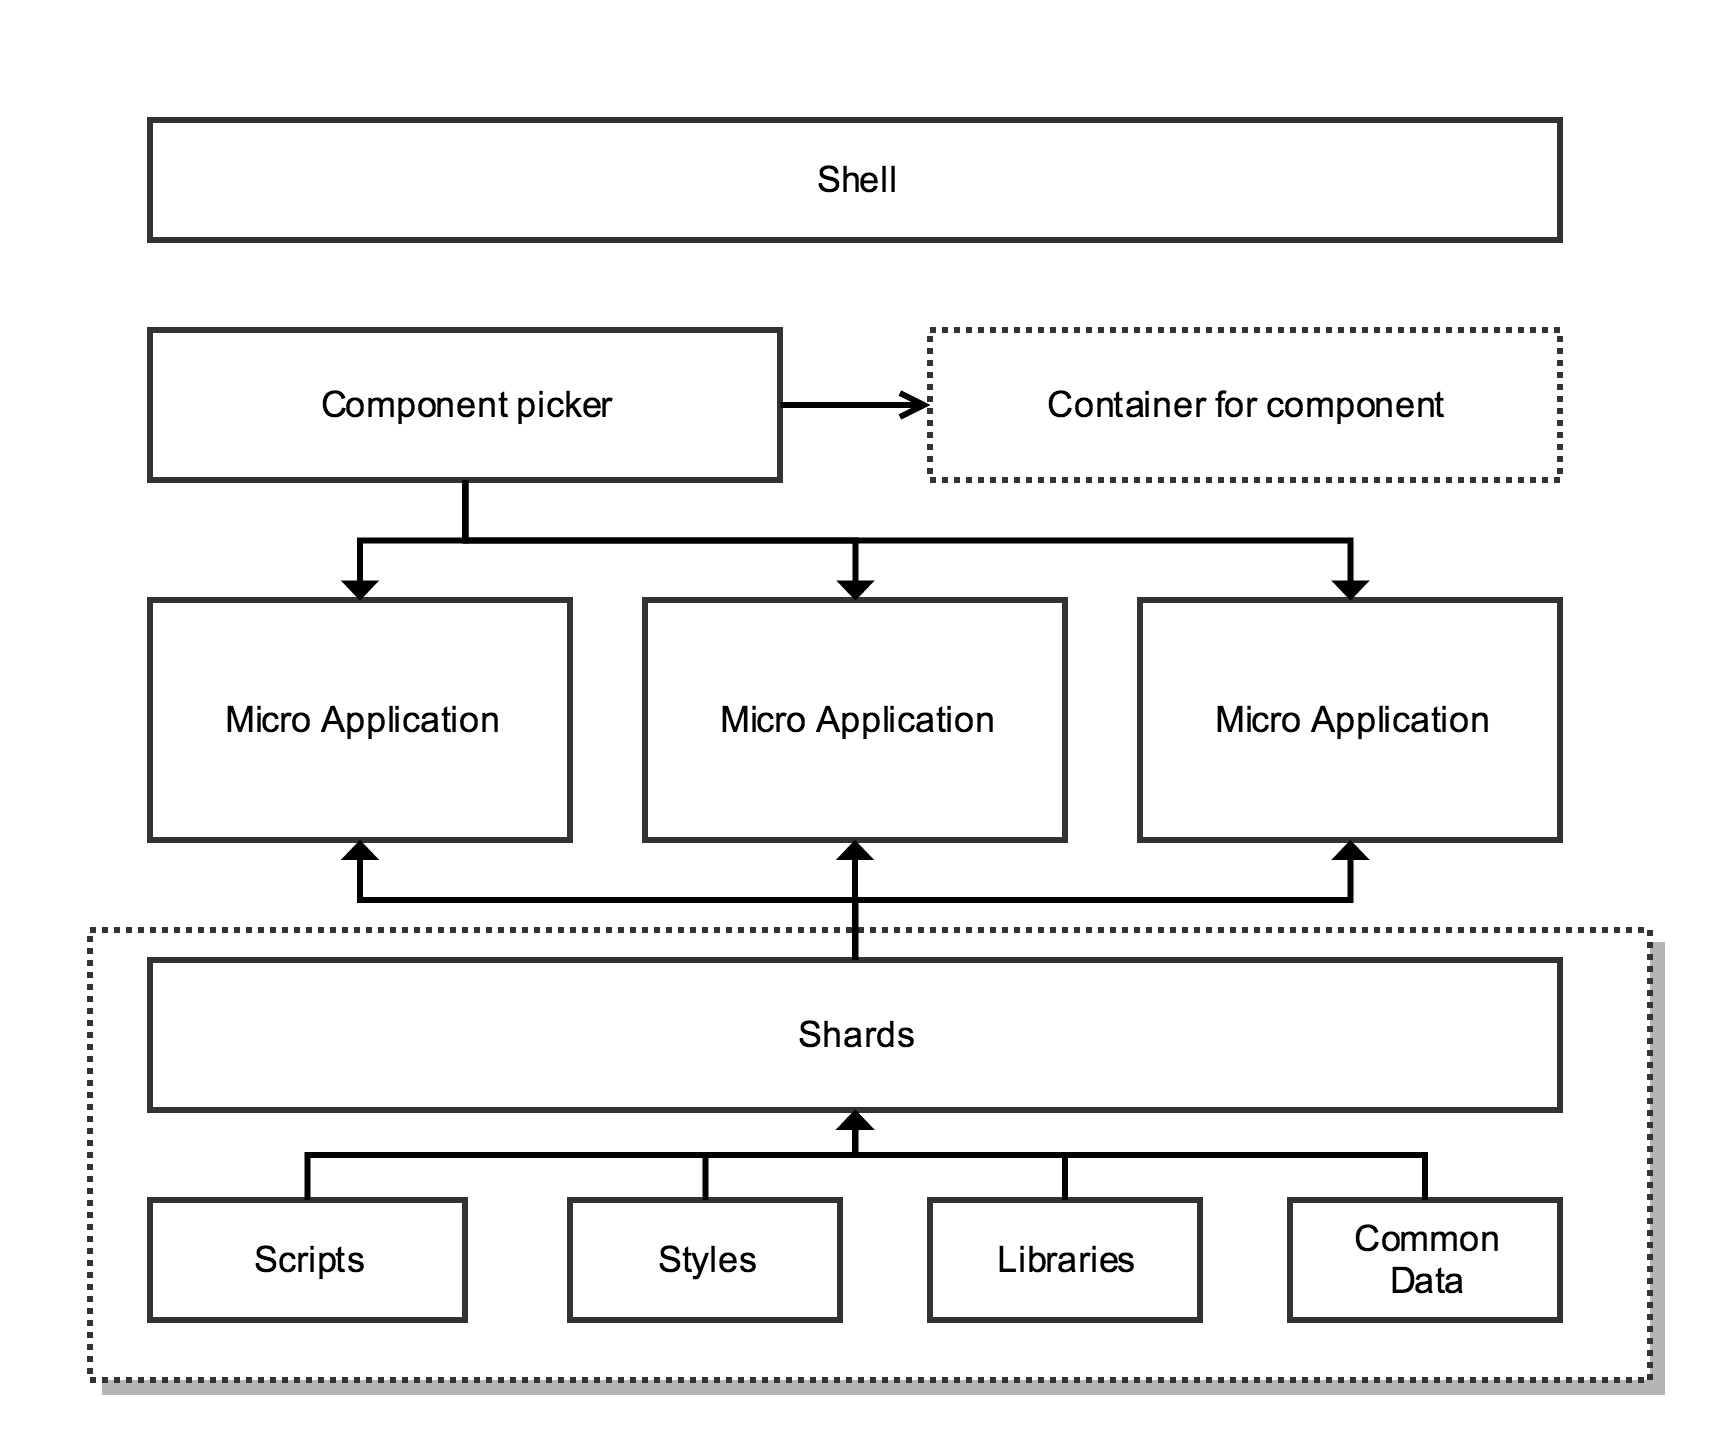
\includegraphics[width=\linewidth]{components/2/frontend_arch.png}
  \caption{Microservices approach in frontend application}
  \label{fig:frontend_arch}
\end{center}
\end{figure}


Microservices approach in frontend application is shown in figure \ref{fig:frontend_arch}. This breaks the entire application into small micro applications.

\begin{itemize}
\item \emph{Shell.}  is a top-level component, which wraps the Components picker and Container for the component. It contains the  application configuration.
\item \emph{Component picker.} Is a router, which manages the micro applications. 
\item \emph{Container for Component.} Container, where the component will be injected.
\item \emph{Micro Application.} Independent application, which can be written in any programming language but has to use one of the shards.
\item \emph{Shards.} Is a code base, which is shared between Micro Applications. Shards can have multiple levels. 
\end{itemize}
 

The central concept of the application is to support the Software as a Service (SaaS) and Platform as a Service (PaaS) distributions \cite{Walraven2014}.  N2Sky consists of two modules: administration module and main application module as shown in figure \ref{fig:modular_design}.

\begin{figure}[H]
\begin{center}
  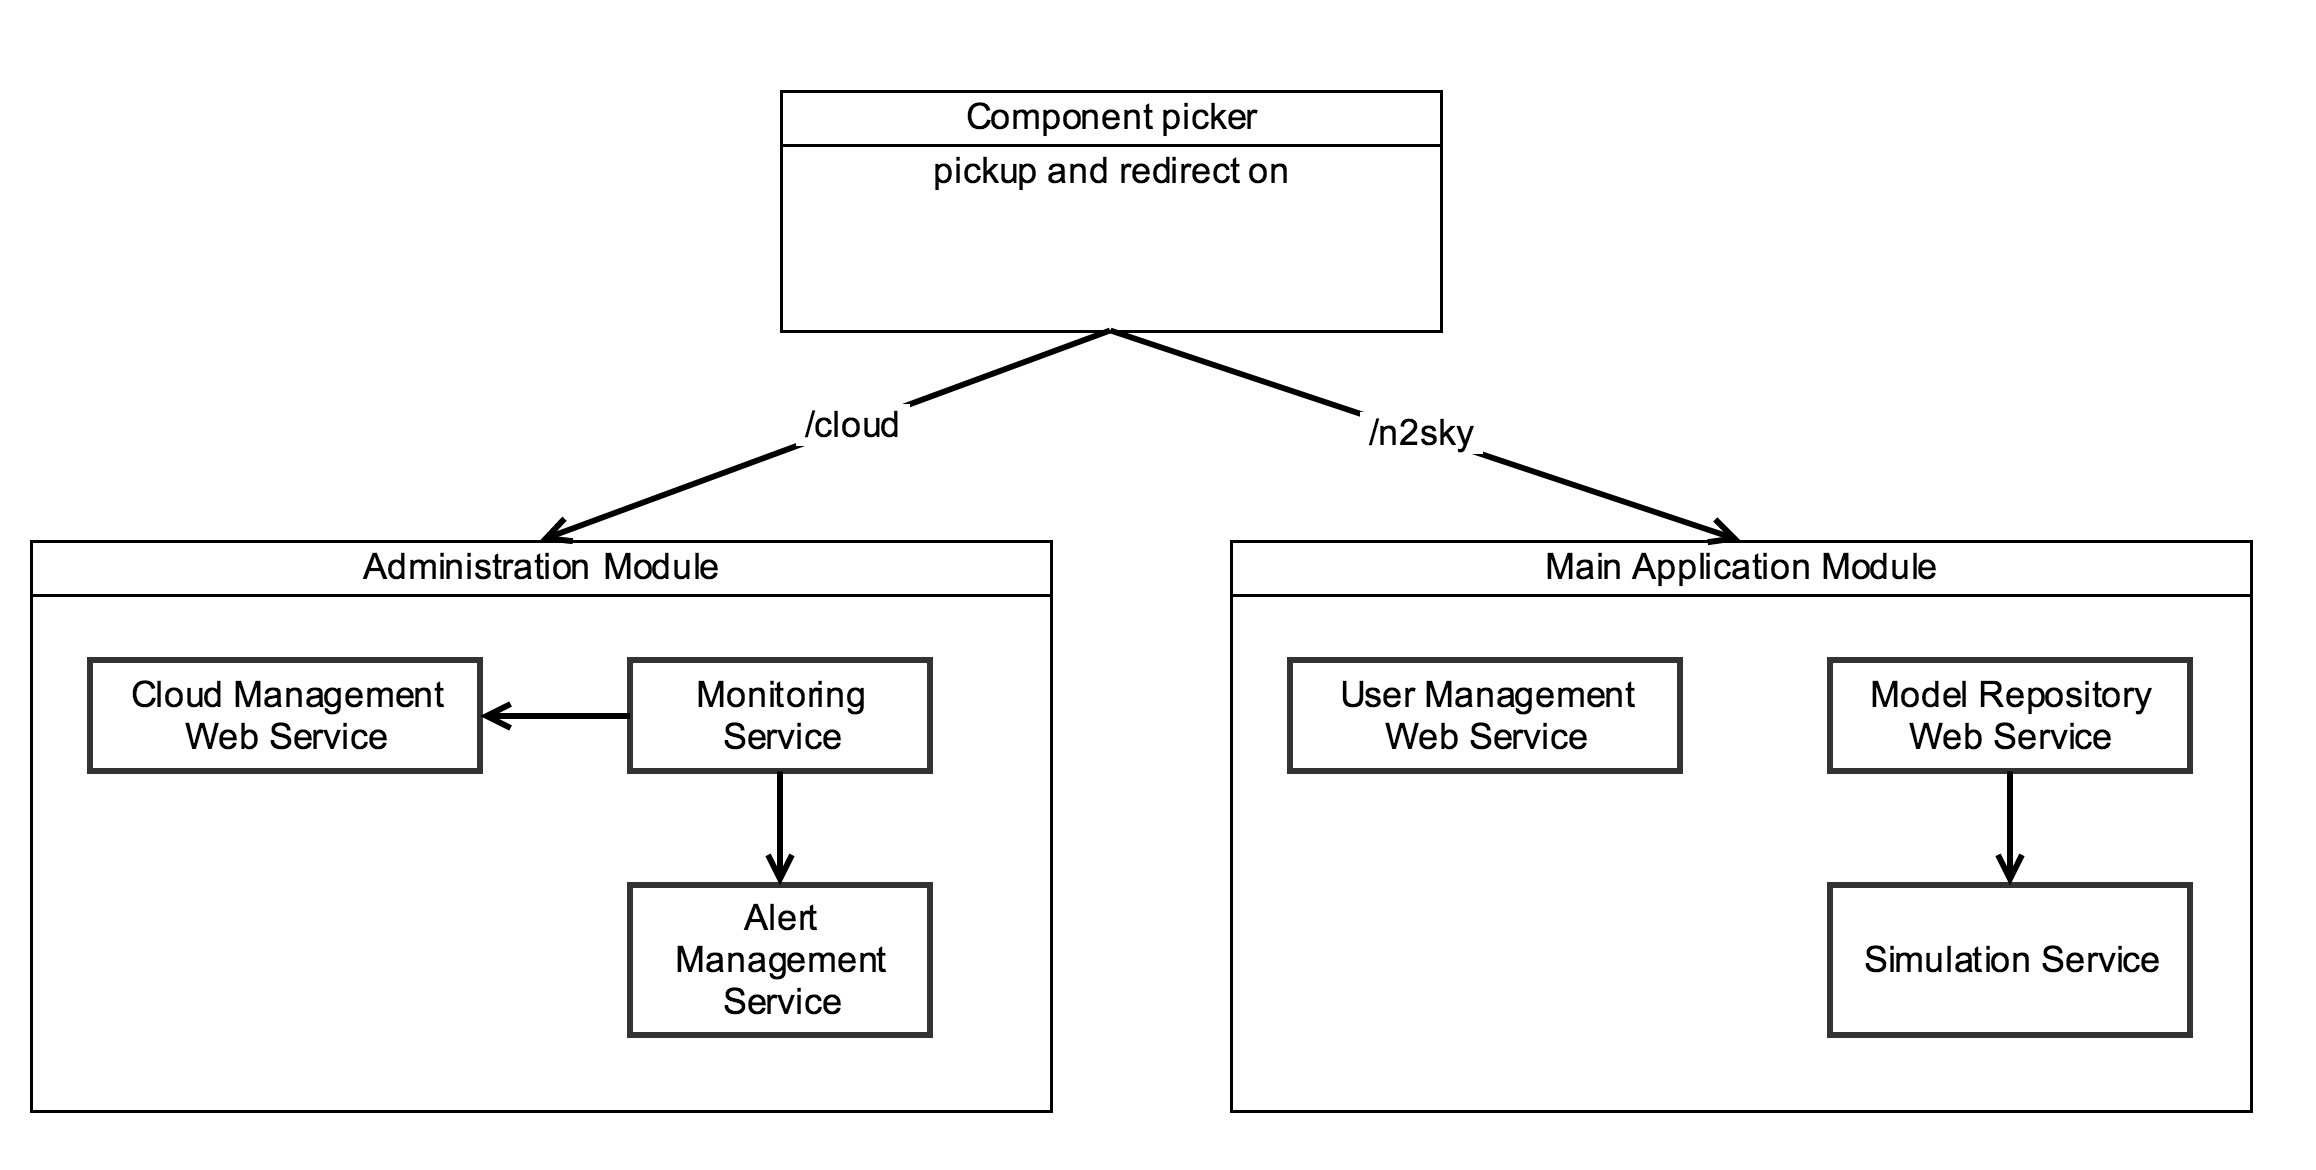
\includegraphics[width=\linewidth]{components/2/redirector.png}
  \caption{N2Sky frontend application and its services}
  \label{fig:modular_design}
\end{center}
\end{figure}

\begin{itemize}
\item \emph{N2Sky component picker.} When the user is located in to the N2Sky web portal, first he will be dealing with the component picker. The component picker is a small service, which redirects the user depending on the URL path.
\begin{itemize}
\item \emph{/cloud} redirects to "Administration module"
\item \emph{/n2sky} redirects to "Main application module"
\end{itemize}


\item \emph{Administration module} The administration module allows the system administrator to control the environment. The module supports OpenStack and Cloudify monitoring. Managing is possible through the application dashboard. It also contains custom monitoring and an alerting management system, which can be installed on any server within the N2Sky user interface. The administration module implements PaaS. It is fully configurable and wrapped into the open source project in order to make the module accessible to the third-party applications. 
\item \emph{Main application module} The main application module is the central module of N2Sky. Within this module, users can use, train and test existing neural networks. It is possible to reuse the neural network paradigms and create own neural networks. N2Sky allows deploying own networks and store data in the cloud. Module services are supporting the SaaS distribution. Experts can use an application directly through the N2Sky API or they can integrate N2Sky services into their own application. 
\end{itemize}


\subsubsection{The Sample Workflow}


The central figure is the N2Sky Web/Mobile portal. It is the frontend application of the N2Sky, which consist of modular subsystems. Since the frontend application has responsive design, it supports desktop devices as well as mobile devices. 
To support the Software as a Service distribution, every web service can work independently. This means that the stakeholders can use N2Sky via web portal as well as use N2Sky API.
N2Sky API allows stakeholders to:

\begin{itemize}
\item Authorise in the System
\item Create new neural from existing paradigm
\item Deploy own neural networks on N2Sky environment 
\item Perform training against own as well published neural network
\item Perform testing against trained models
\end{itemize}

Almost everything is available for arbitrary stakeholders, except cloud services. In order to use cloud service as a service, the user has to install it on his own cloud environment. This approach supports the Platform as a Service distribution. Cloud services are only available for system administrator and granted users. 


\begin{figure}[htbp]
\begin{center}
  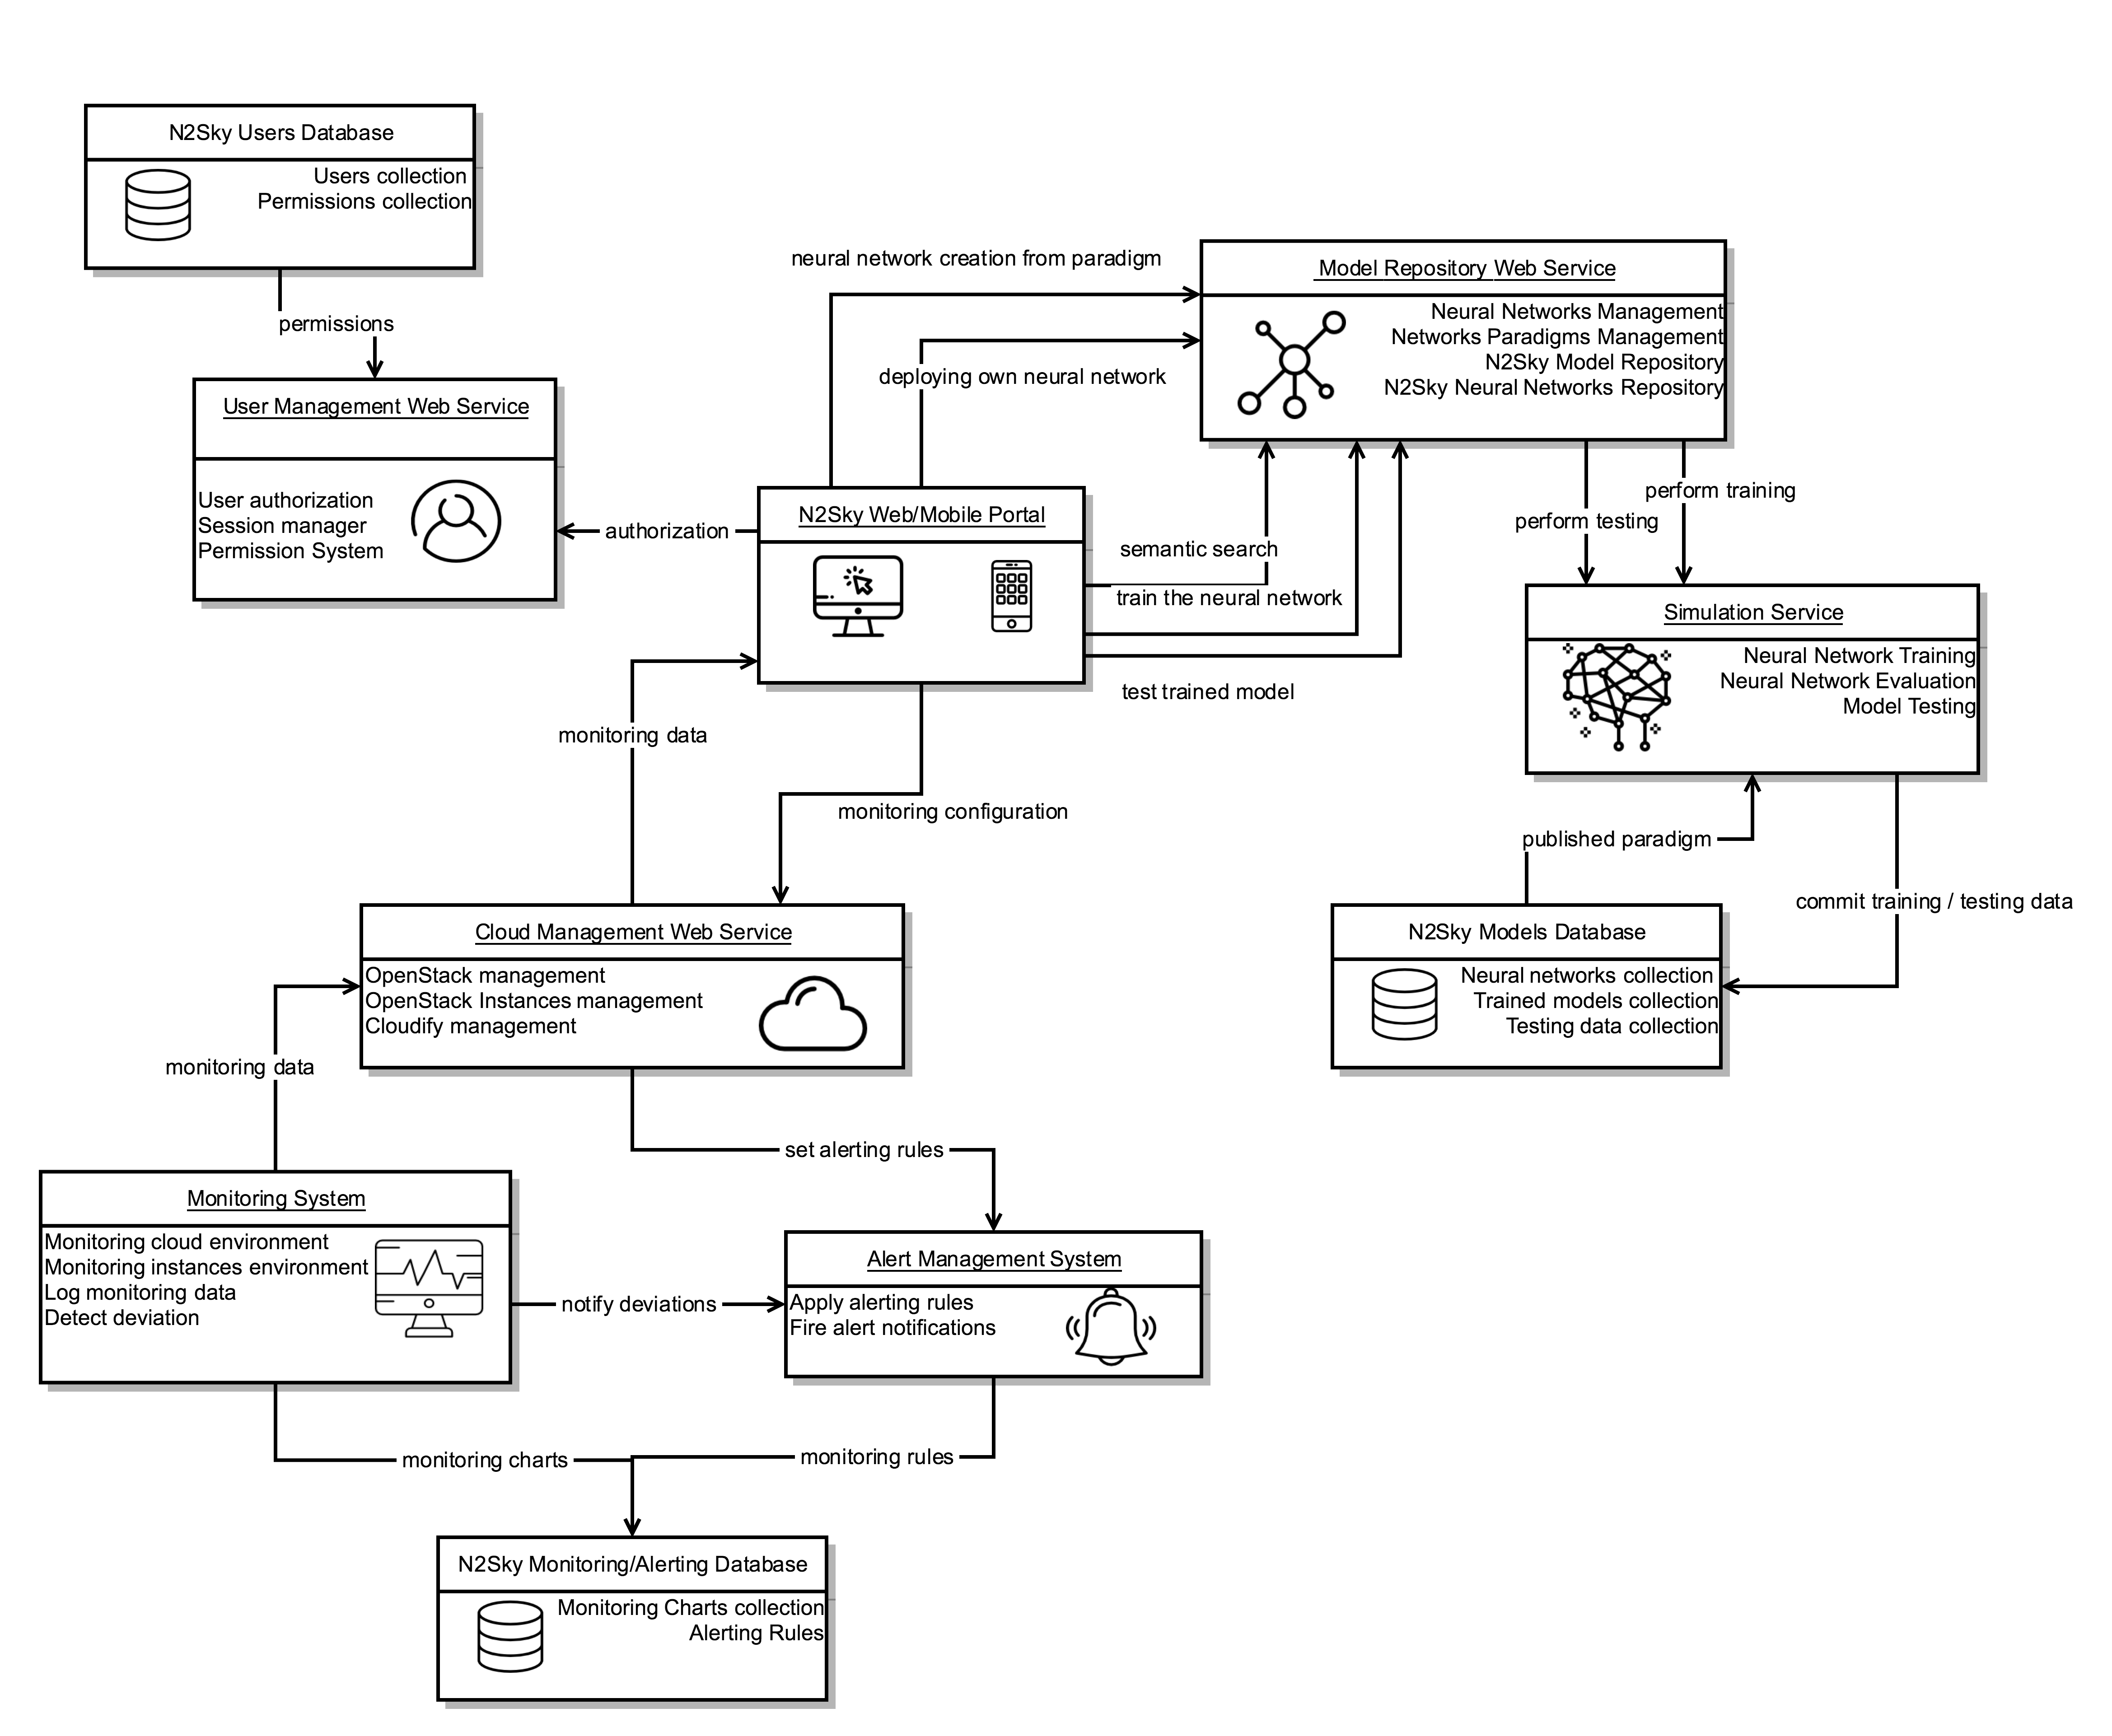
\includegraphics[width=\linewidth]{components/2/new_arch.png}
  \caption{The sample workflow}
  \label{fig:newarch}
\end{center}
\end{figure}


The sample workflow overview, which shown in figure \ref{fig:newarch} represents microservices architecture in action:


\begin{enumerate}
\item \emph{Contributor User}
\begin{enumerate}
\item The Contributor user authorizes the N2Sky portal using his browser on desktop PC or mobile device. He will be redirected to his own dashboard according to permissions, which will be received from User Management Web Service. 
\item The user describes his own neural network paradigm using the ViNNSL template and deploying it in the N2Sky cloud. 
\item The Contributor user performs training of his neural network using the N2Sky platform. Since the user is an expert, he can perform this operation using Simulation Service via Model Repository Web Service API.
\item The user publishes his paradigm via N2Sky UI or the available API. 
\item The Contributor user will be awaiting until other N2Sky users use his neural network paradigm in order to monitor the behavior of the neural network. 
\item The user modifies, redeploys and retrains his neural network after the first results. 
\end{enumerate}
\item \emph{Neural Network Engineer User}
\begin{enumerate}
\item The neural network engineer user authorizes the N2Sky portal using his browser on desktop PC or mobile device. He will be redirected to his own dashboard according to permissions, which will be received from User Management Web Service. 
\item From the dashboard, the user creates a neural network from existing paradigms using Model Repository Web Service.
\item The user performs training against his newly created neural network using the N2Sky platform. 
\item If the user is satisfied with a trained model, he can perform testing using the N2Sky platform. 
\item The neural network engineer user can publish his neural networks and trained models in order to make it available for other N2Sky users. 
\end{enumerate}
\item \emph{Arbitrary User}
\begin{enumerate}
\item The arbitrary user authorizes the N2Sky portal using his browser on desktop PC or mobile device. He will be redirected to his own dashboard according to permissions, which will be received from User Management Web Service. 
\item Since the user does not much knowledge in the neural network field, he performs a semantic search in order to find some neural network as well as trained models according to his needs.
\item The user copies existing neural network and trained models into his project. 
\item The user performs training from the N2Sky platform against copied neural network with the default input parameters data.
\item The user evaluates trained neural network models with the default parameters. 
\end{enumerate}
\item \emph{System Administrator}
\begin{enumerate}
\item The system administrator authorizes the N2Sky portal using his browser on desktop PC or mobile device. He will be redirected to the administration dashboard.
\item The user observes the cloud environment.
\item The system administrator creates the new monitoring chart with specific metrics and adds it to the administration dashboard.
\item The user creates alert against newly created monitoring.
\item The user is notified by the Alert Management System, that a specific event occurs.
\end{enumerate}
\end{enumerate}


\subsubsection{Technology Stack}\label{Technology Stack}

N2Sky today is the cross-platform handy application with a responsive design. Creating an own framework from scratch would be time-consuming. To build a cross-platform framework just for N2Sky is also absurd. After some research on the most popular and common used frontend frameworks, the following candidates were listed: 

\begin{description}
\item[Vaadin.] Java framework, which compiles Java code into JavaScript components. Vaadin supports cross-platform applications, but not fully. It is possible to wrap an application into the container and deploy it only as an Android application.

\begin{itemize}
\item \emph{Benefits.} Easy to develop in Java. The developer does not have to think about JavaScript functionality. There a dozen of predefined components like buttons, input fields, frames etc. Customisation is also possible. 
\item \emph{Obstructions.} The deployment process is a blockage process. There is no "hot redeployment" available. Even if the developer might save time from the build components in Java, he will lose more time by continuous redeployment. 

Java applications need servers which supports JVM, meaning that the server should have much more memory than some other frameworks, which is written in JavaScript language.  
\end{itemize}

\item[ReactJS.]  JavaScript framework, which supports JSX programming language. 
\begin{itemize} 
\item \emph{Benefits.} The main idea is to write HTML code in JavaScript. ReactJS supports hot redeployment. The React-Native extension for this framework allows wrapping the whole application in a mobile as well as in a desktop application.
\item \emph{Obstructions.} Difficulties supporting big projects. JSX is not a type-safe programming language. Exception handling also needs to be done by the developer.  
\end{itemize}
\item[AngularJS.] JavaScript framework, which supports TypeScript programming language.
\begin{itemize} 
\item \emph{Benefits.} The main idea is to write JavaScript code in HTML.  AngularJS same as ReactJS supports hot redeployment. It does not have native support for all mobile devices but is possible to wrap it using the IONIC framework. 
\item \emph{Obstructions.}  AngularJS compiles TypeScript code into the JavaScript core and sometimes the compilation fails because TypeScript is a new language and it is not fully adapted for browsers. 
\end{itemize}
\end{description}
 
 Vaadin does not fit the N2Sky needs, but AngularJS and ReactJS could both perfectly fit. These frameworks are written in JavaScript and have big corporations behind: AngularJS was developed by Google and ReactJS was developed by Facebook. Since N2Sky has to support a fully cross-platform architecture, it was decided to choose ReactJS. With this framework, N2Sky has great potential to be a multi-platform application in the future. 
 

Furthermore, the backend has the microservices architecture to support scalability. By choosing the JavaScript framework for frontend, it makes sense to use the same in backend as well, so that server would be small and fast. Each one of the microservices is developed on NodeJS Framework server, which implies efficiency and lightweight. 

N2Sky is a cloud-based system. OpenStack cloud platform supports this approach. Since N2Sky uses OpenStack API for the administration dashboard, the original dashboard was no more needed. Every backend and frontend service is deployed on OpenStack instances. Every instance is absolutely scalable, which allows finding the best environment for every service. 

Each OpenStack instance is a server with either Debian or Ubuntu operational system. Every instance, as well as OpenStack itself, has to be monitored 24/7, that is why there exists a Monitoring Management System. The basis of this system is Prometheus monitoring system, which gives full access to all information on any installed server. Prometheus has an open API, which is used by N2Sky. Using Prometheus, there were charts and graphs developed and integrated into N2Sky. The Alert Management System, which is a part of N2Sky, is also using the Prometheus API in order to detect the deviation and notify if an event occurred.

As a database, it was decided to choose the NoSQL one. There were two NoSQL databases under consideration ElasticSearch and MongoDB. 
ElasticSearch supports indexes. It is possible to configure this index, so that is impossible to insert something which is not mapped by the index. MongoDB does not use the index approach, but a MongoDB client supports the schema. It was decided to use this MongoDB schema and map the ViNNSL schema to it in order to make it more understandable for other developers. 

For continuous delivery and quick configuration, it was decided to use Jenkins Continuous Integration system. In case of a whole unreachable system, every service can be restored with a Jenkins Profiles.


